\subsection{Design der Erklärungen}

Das Gestalten der Erklärungen ist mit mehreren Design-Mockups umgesetzt worden. Grundsätzlich ist für die funktionalen Anforderungen 1-4 jeweils ein Erklärungstyp entstanden. Wie aus Protokoll des durchgeführten Workshops zu entnehmen ist, wurden bereits in diesem einige Ideen für Erklärungen auf Basis der Vorschläge zur Umsetzung von Erklärungen aus dem Modell für Erklärungen entwickelt (\textit{Characteristics}).

Außerdem wurden bei der Umsetzung die Zusammenhänge zwischen den Eigenschaften von Erklärungen auf Qualitätsaspekte sowie die Heuristiken für das Design von Erklärungen beachtet. Insbesondere wurde darauf geachtet, dass die Erklärungen dezent sind, sodass sie möglichst keinen negativen Einfluss auf die \textit{Usability} haben. Längere Erklärungen werden nur optional eingesetzt. Auch wurde, wie im Leitfaden vorgeschlagen versucht, für eine Information möglichst hybride Stile zu nutzen, sodass die \textit{End User} diese auf mehrere Weisen erfassen können.

Da eine weitere Empfehlung des Leitfadens die \textit{Context Sensitivity} von Erklärungen betrifft, wird im Folgenden der \textit{Context} von \textit{NUNAV Navigation} beschrieben.
% Die \textit{End User} wurden bereits zuvor beschrieben (siehe \autoref{sec:06_model_evaluation:personas}). 
Grundsätzlich kann im Fall von Navigationsanwendungen zwischen zwei verschiedenen Situationen unterschieden werden. Die erste ist die Nutzung der Anwendung außerhalb der aktiven Navigation. Dies beinhaltet das Auswählen des Ziels, eine Routenübersicht, sowie die Möglichkeit des Startens der Navigation. Hier haben die \textit{End User} keinen Zeitdruck und können sich auf die Interkation mit der Applikation konzentrieren. Trotz dessen wurden die Erklärungen so entwickelt, dass diese von den \textit{End Usern} wie von \citeauthor{chazette_end-users_nodate} sowie \citeauthor{wang_integration_2020} vorgeschlagen, optional angefordert werden müssen \cite{chazette_end-users_nodate,wang_integration_2020}. Folglich wurden für die Anforderungen FR1 und FR2 in diesem \textit{Context} umgesetzt. Grund dafür ist, dass die Informationsmenge zur Erklärung des Routingalgorithmus und der dazugehörigen Daten so groß ist, dass eine Integration in der zweiten möglichen Situation nicht ohne Beeinflussung der Nutzerperformanz möglich ist.

Die zweite Situation ist die aktive Navigation. Während dieser sollten die \textit{End User} so wenig wie möglich abgelenkt werden, da sie der vollen Konzentration auf die Straße bedürfen. Daher sind alle Erklärungen, die während der Navigation den \textit{End Usern} zur Verfügung gestellt werden entgegen der Empfehlung für Interaktionen mit Erklärungen ohne eine Manipulationsmöglichkeit durch die \textit{End User} gestaltet. Da die Anforderungen FR3 und FR4 von einer aktiven Navigation abhängig sind, wurden diese im zweiten \textit{Context} integriert.

Die vier entwickelten Erklärungstypen werden im Folgenden im Detail vorgestellt.

% Grafiken von eingehendem Datenstrom und ausgehenden Datenstrom.
% explain \textit{Affordance}

\subsubsection{Kollaboratives Routing}
\label{sec:user_count_definition}

\paragraph{[FR1]} NUNAV muss den \textit{End Usern} die Möglichkeit bieten, auf eine Erklärung zuzugreifen zu können, die den Routingalgorithmus erklärt.

\bigskip

Wie bereits erläutert ist der Kerngedanke des \textit{NUNAV}-Routingalgorithmus, dass jeder \textit{End User} eine individuell schnellste Route erhält und dabei nicht zwangsweise Hauptverkehrsstraßen nutzt. Folglich ist für diese erste Anforderung eine Erklärung entworfen worden, die das Kollaborative Routing erklärt.

Wie bei genauerem Einblick in das Feedback von \textit{End Usern} auffällt, ist eines der Grundprobleme, dass ihnen das Verständnis fehlt, dass sie vernetzt mit anderen Nutzern von \textit{NUNAV} kollaborativ navigiert werden. Da dies einer der Hauptunterschiede zu anderen Navigationsanbietern ist, sind Erklärungen die diesen Punkt betreffen vor allem für Erstnutzer wie Ayla wichtig. Um den Nutzern einen Einblick in diese Abhängigkeit von anderen Verkehrsteilnehmern zu geben, wird die aktuelle Anzahl der Nutzer, welche sich in einem Bereich, der die eigene Route beeinflusst, befinden angezeigt. Diese Berechnung dieser Zahl ist eine Annäherung, da sich nicht genau bestimmen lässt, welche Fahrzeuge auf der Straße einen realen Einfluss auf die eigene Navigation haben. Die Annäherung wurde allerdings als ausreichend befunden da, wie im Leitfaden beschrieben wird, die Richtigkeit der Erklärung keinen Einfluss auf die \textit{Transparency} hat, welche Ziel dieser Anforderung ist. In einem ersten Entwurf wurden alle aktiven Nutzer im System als Zahl angenommen. Dies wurde allerdings verworfen, da Nutzer aus dieser Zahl wenig Informationen über den unmittelbaren Einfluss auf für eigene Navigation bekommen.

Die Anzahl der Nutzer wurde von einem Backend-Team bei Graphmasters zur Verfügung gestellt, die restliche Umsetzung in \textbf{BFF} und App ist im Rahmen dieser Arbeit erfolgt. Für die Anzeige der Nutzerzahl wurden verschiedene Positionen im User Interface ausprobiert, wie in \autoref{fig:prototype_collaborative_routing} zu erkennen ist. Für die finale Version ist die Entschiedung gefallen, da an dieser Stelle bereits andere Informationen als sogenanntes \textit{Growl} angezeigt werden und diese Stelle zur Anzeige kurzer Informationen somit im Rahmen der \textit{Usabiltiy} bereits erfolgreich ohne negatives Feedback genutzt wird. Das \textit{Growl} ist in den Screenshots (a) und (b) der Abbildung rot umrahmt.

Eine Erklärung des Algorithmus ist in zwei verschiedenen Granulariätsstufen umgesetzt worden. Tippen \textit{End User} auf das \textit{Growl} mit der Anzahl der Nutzer gelangen sie zu einer kurzen Erklärung (siehe \autoref{fig:prototype_collaborative_routing}, (c)). Ursprünglich war der Text \glqq In den letzten 15 Minuten haben wir anonyme Verkehrsdaten von x Nutzern in deiner Umgebung erhalten\grqq{}. Nachdem zu diesem Text intern bei Graphmasters das Feedback kam, dass dieser zu technisch bzw. datengetrieben ist, wurde dieser so geändert, dass der direkte Einfluss auf die \textit{End User} klar wird (siehe \autoref{fig:prototype_collaborative_routing}, (c)).

Als weitere Erklärungsmöglichkeit können die \textit{End User} mittels \glqq Mehr erfahren\grqq{} zu dem entsprechenden Hilfe-Center-Artikel springen (siehe \autoref{sec:help_center_collaboratrive_routing}). Eine Verknüfung aus der App heraus direkt zum Hilfe-Center gab es an dieser Stelle noch nicht.

\begin{figure}[htb!]
    \centering
    \subfloat[1. Prototyp zur Positionierung der Nutzerzahl]
    {
        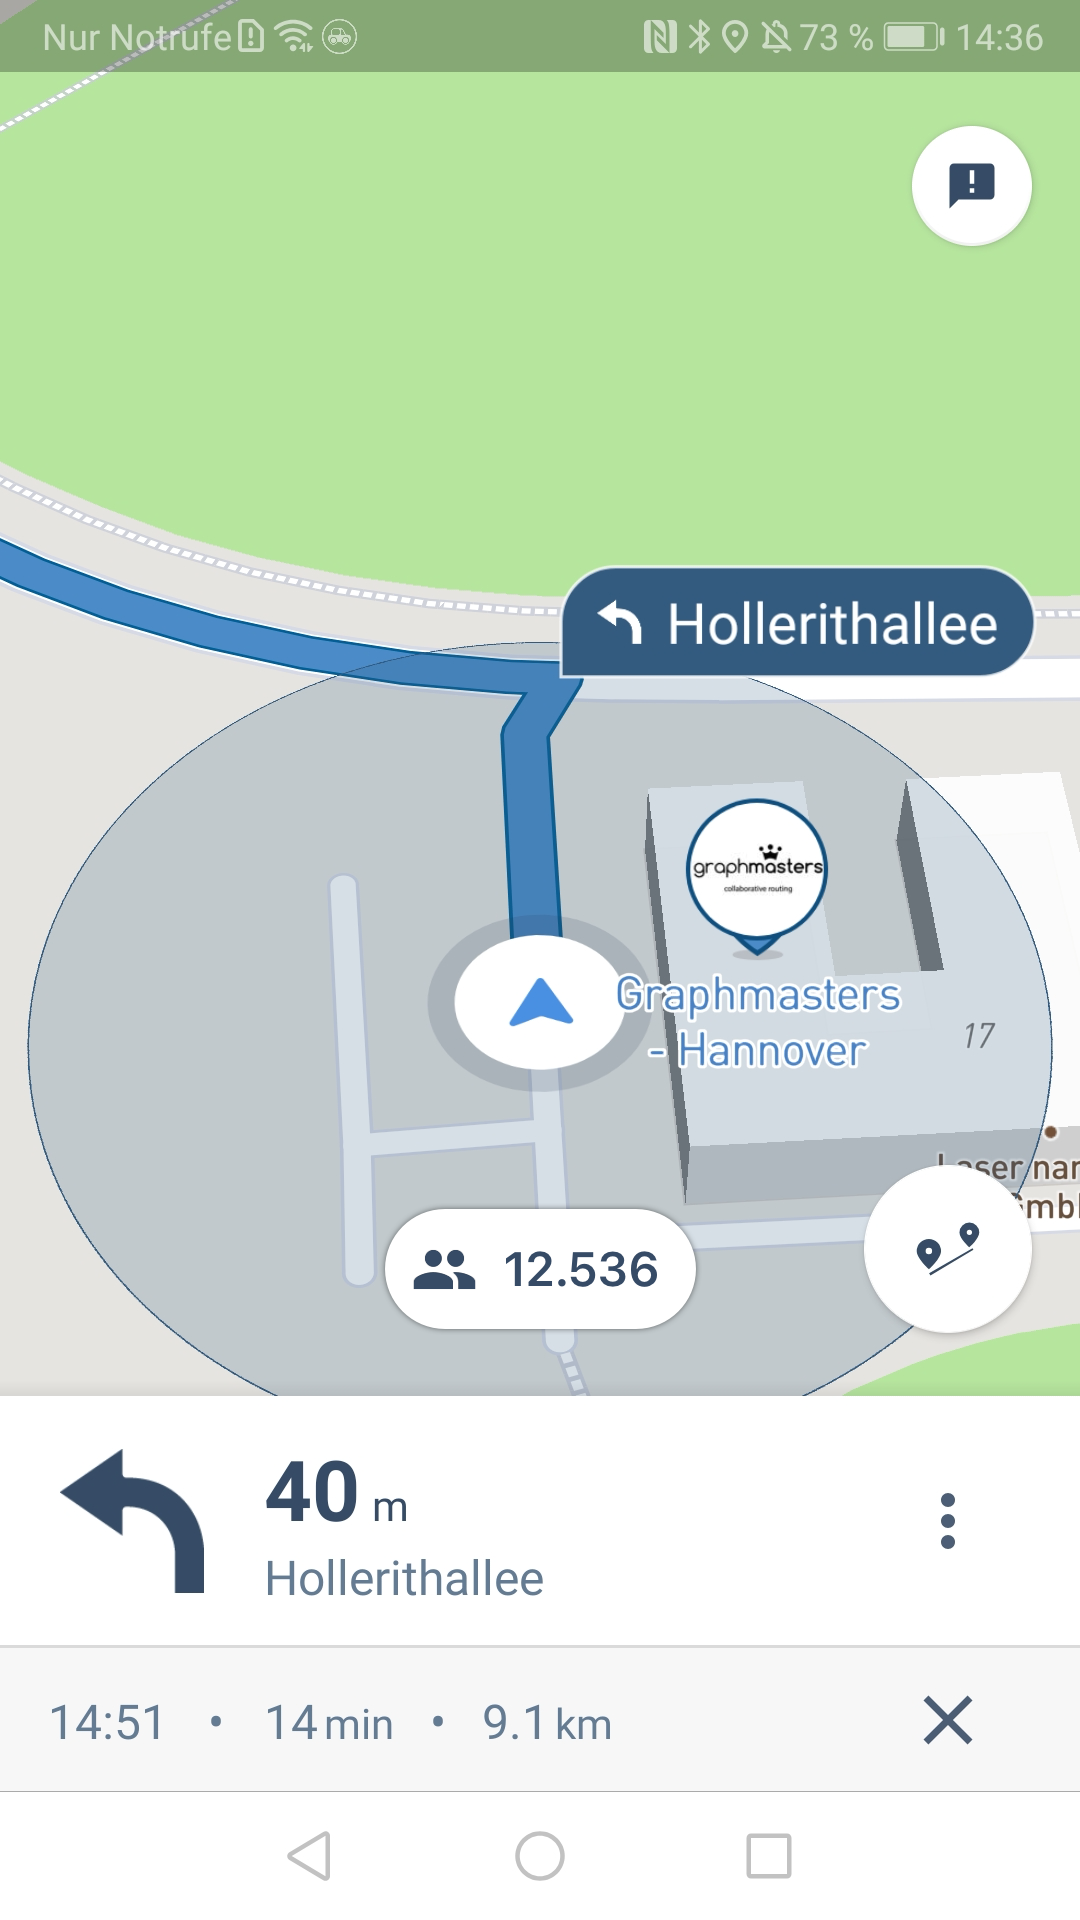
\includegraphics[width=.27\linewidth]{contents/06_model_evaluation/01_integration/res/01_collaborative_routing/prototype_1.png}
    }
    \hspace{.055\linewidth}
    \subfloat[Finales Design der Positionierung der Nutzerzahl]
    {
        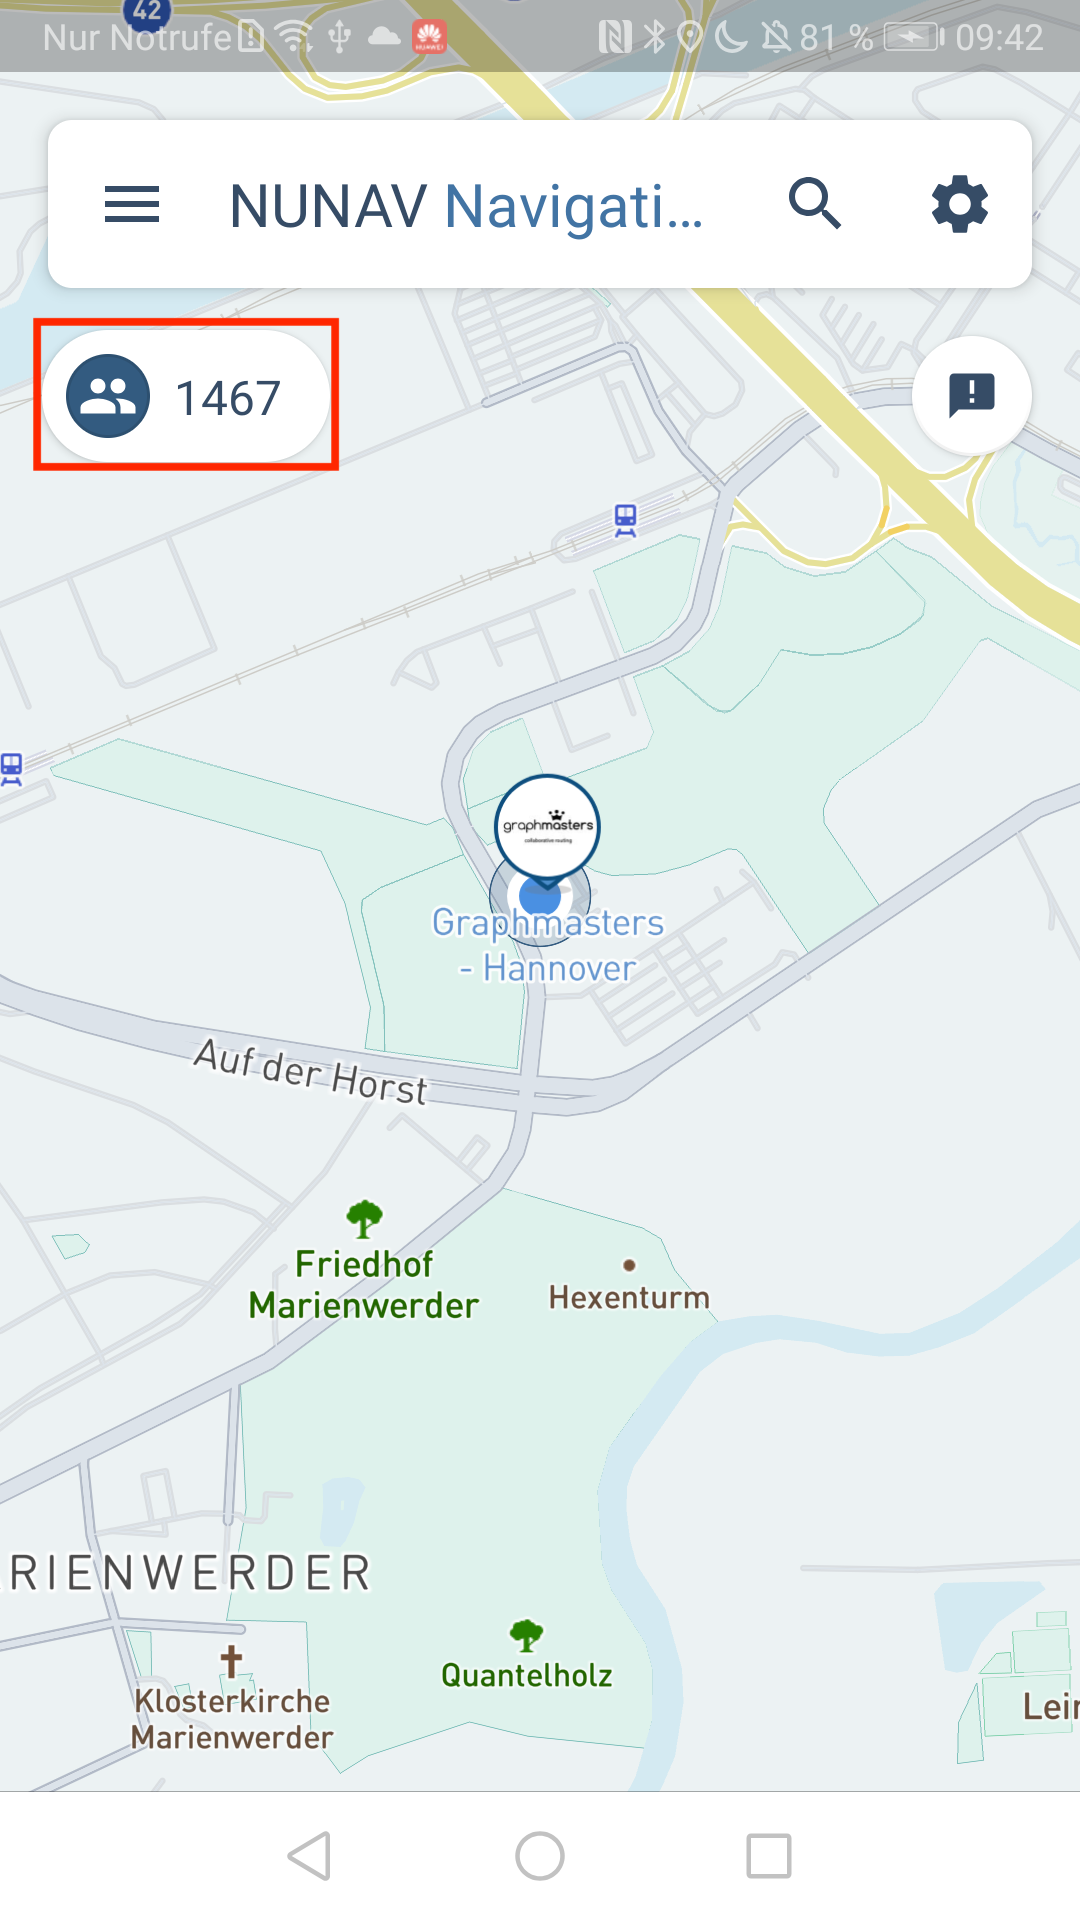
\includegraphics[width=.27\linewidth]{contents/06_model_evaluation/01_integration/res/01_collaborative_routing/final_1.png}
    }
    \hspace{.055\linewidth}
    \subfloat[Finales Design der kurzen Erklärung zum kollaborativen Routing]
    {
        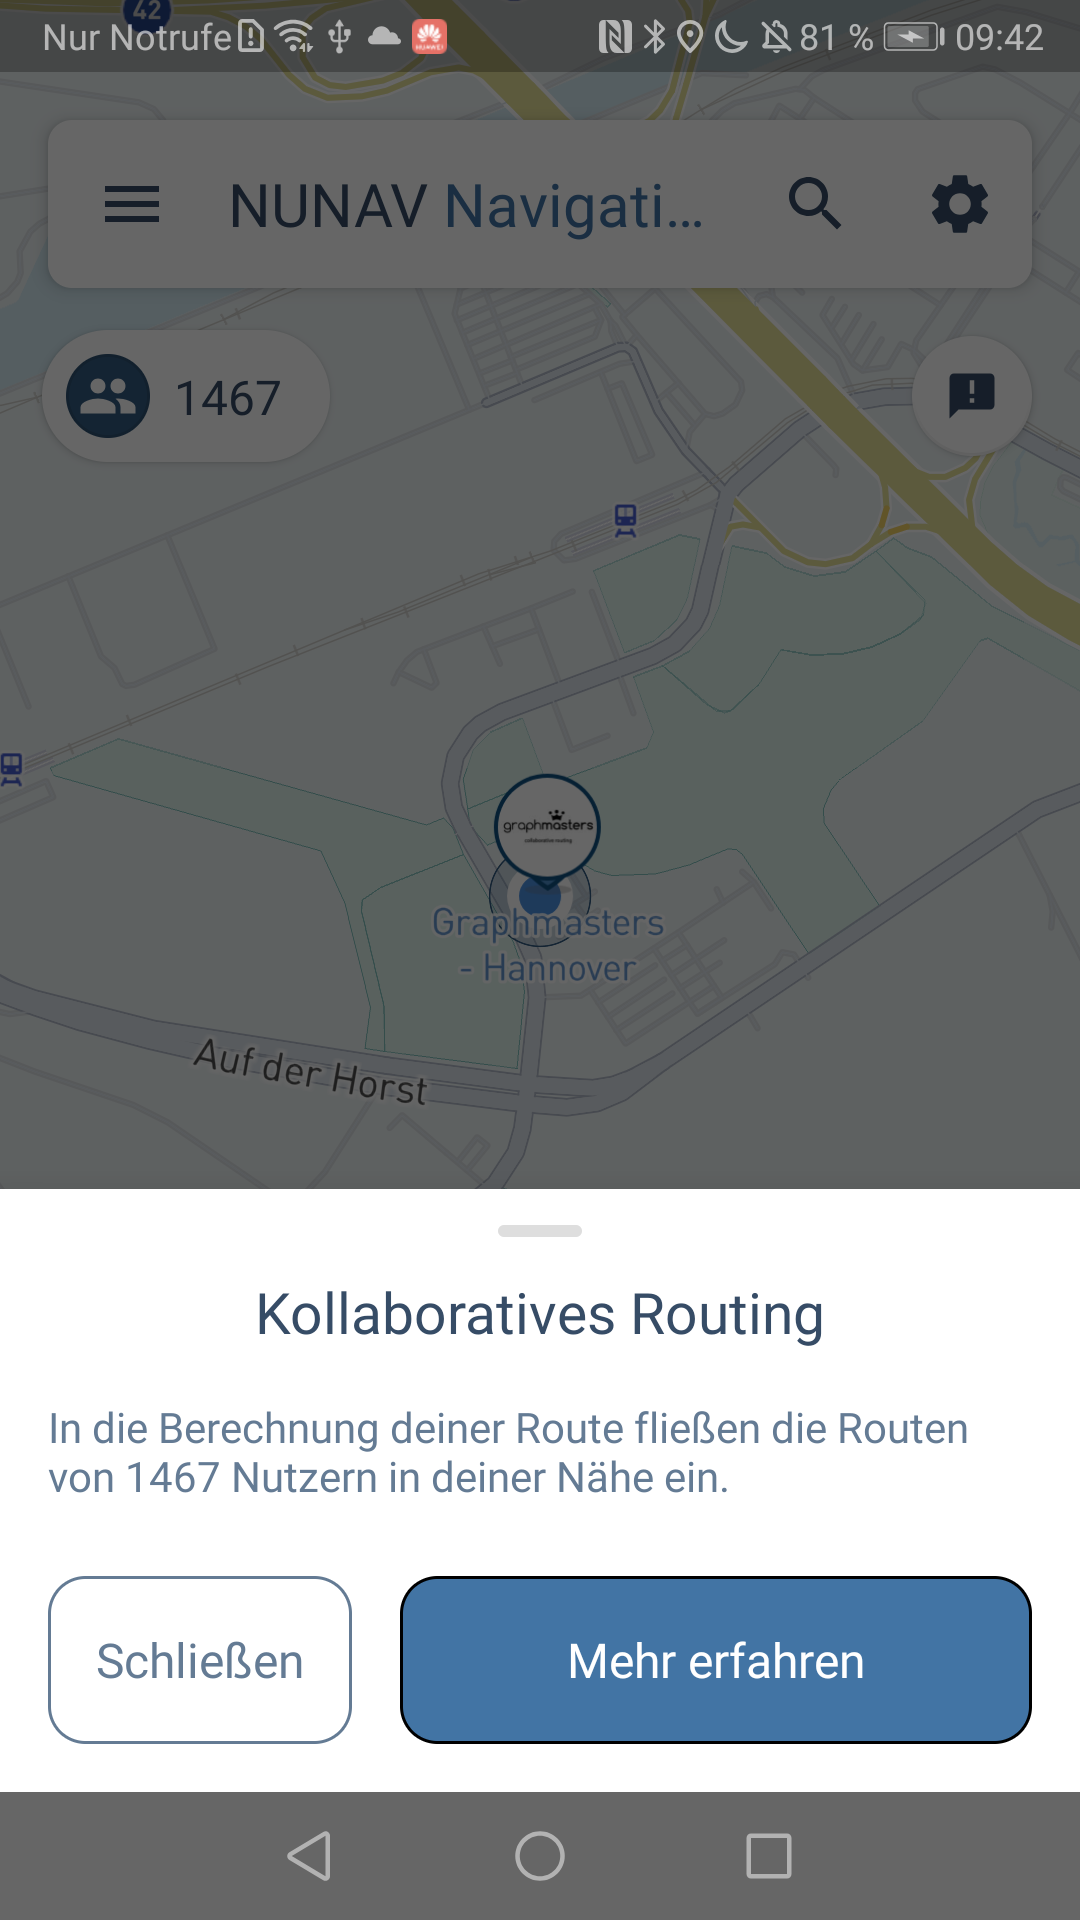
\includegraphics[width=.27\linewidth]{contents/06_model_evaluation/01_integration/res/01_collaborative_routing/final_2.png}
    }
    \caption{Prototyp und finale Designs für die Erklärung zum kollaborativem Routing}
    \label{fig:prototype_collaborative_routing}
\end{figure}

\subsubsection{Einflüsse auf die Routenberechnung}

\paragraph{[FR2]} \textit{NUNAV Navigation} muss den \textit{End Usern} die Möglichkeit bieten, abzurufen, welche Informationen zu Verkehrsereignissen (z.B. Verkehrsfluss, Sperrungen, Baustellen, Staus) in den Algorithmus einfließen.

\bigskip

Auf der Karte, welche das Hauptinteraktionselement von \textit{NUNAV Navigation} darstellt, sind Sperrungen, Baustellen und Staus bereits eingezeichnet. Wie aus dem Nutzerfeedback hervorgeht reichen diese \textit{Context}-Informationen allerdings für das Verständnis der \textit{End User} nicht aus. Daher wurde ein neuer Hilfe-Center-Artikel im Rahmen dieser Arbeit zu diesem Thema angelegt (siehe \autoref{sec:help_center_routing_data}). Dieser Artikel ist für Nutzer geeignet, welche NUNAV zum ersten Mal wie Ayla oder noch nicht lange wie Michael verwenden. So können sie sich anhand der Daten auf der Karte im Anschluss an das Lesen des Artikels die verschiedenen Routen besser erklären.

Dieser Beitrag wurde ebenfalls vor dem Start der Navigation erreichbar gemacht. Um die Standardkartenansicht nicht durch mehrere Möglichkeiten zum Aufrufen von Hilfe-Center-Artikeln zu überladen, wurde die Möglichkeit, zu dieser Erklörung zu gelangen, in die Routen-Vorschau integriert. Auch für diese wurden mehrere Prototypen erstellt, wobei bei der finalen Entscheidung darauf geachtet wurde, dass die Aufrufmöglichkeit nicht zu viel Platz einnimmt und der Text neugierig macht. Die verschiedenen Prototypen sind in \autoref{fig:prototype_routing_explanation} zu sehen.

\begin{figure}[htb!]
    \centering
    \subfloat[1. Prototyp zur Positionierung des Aufrufs der Erklärung]
    {
        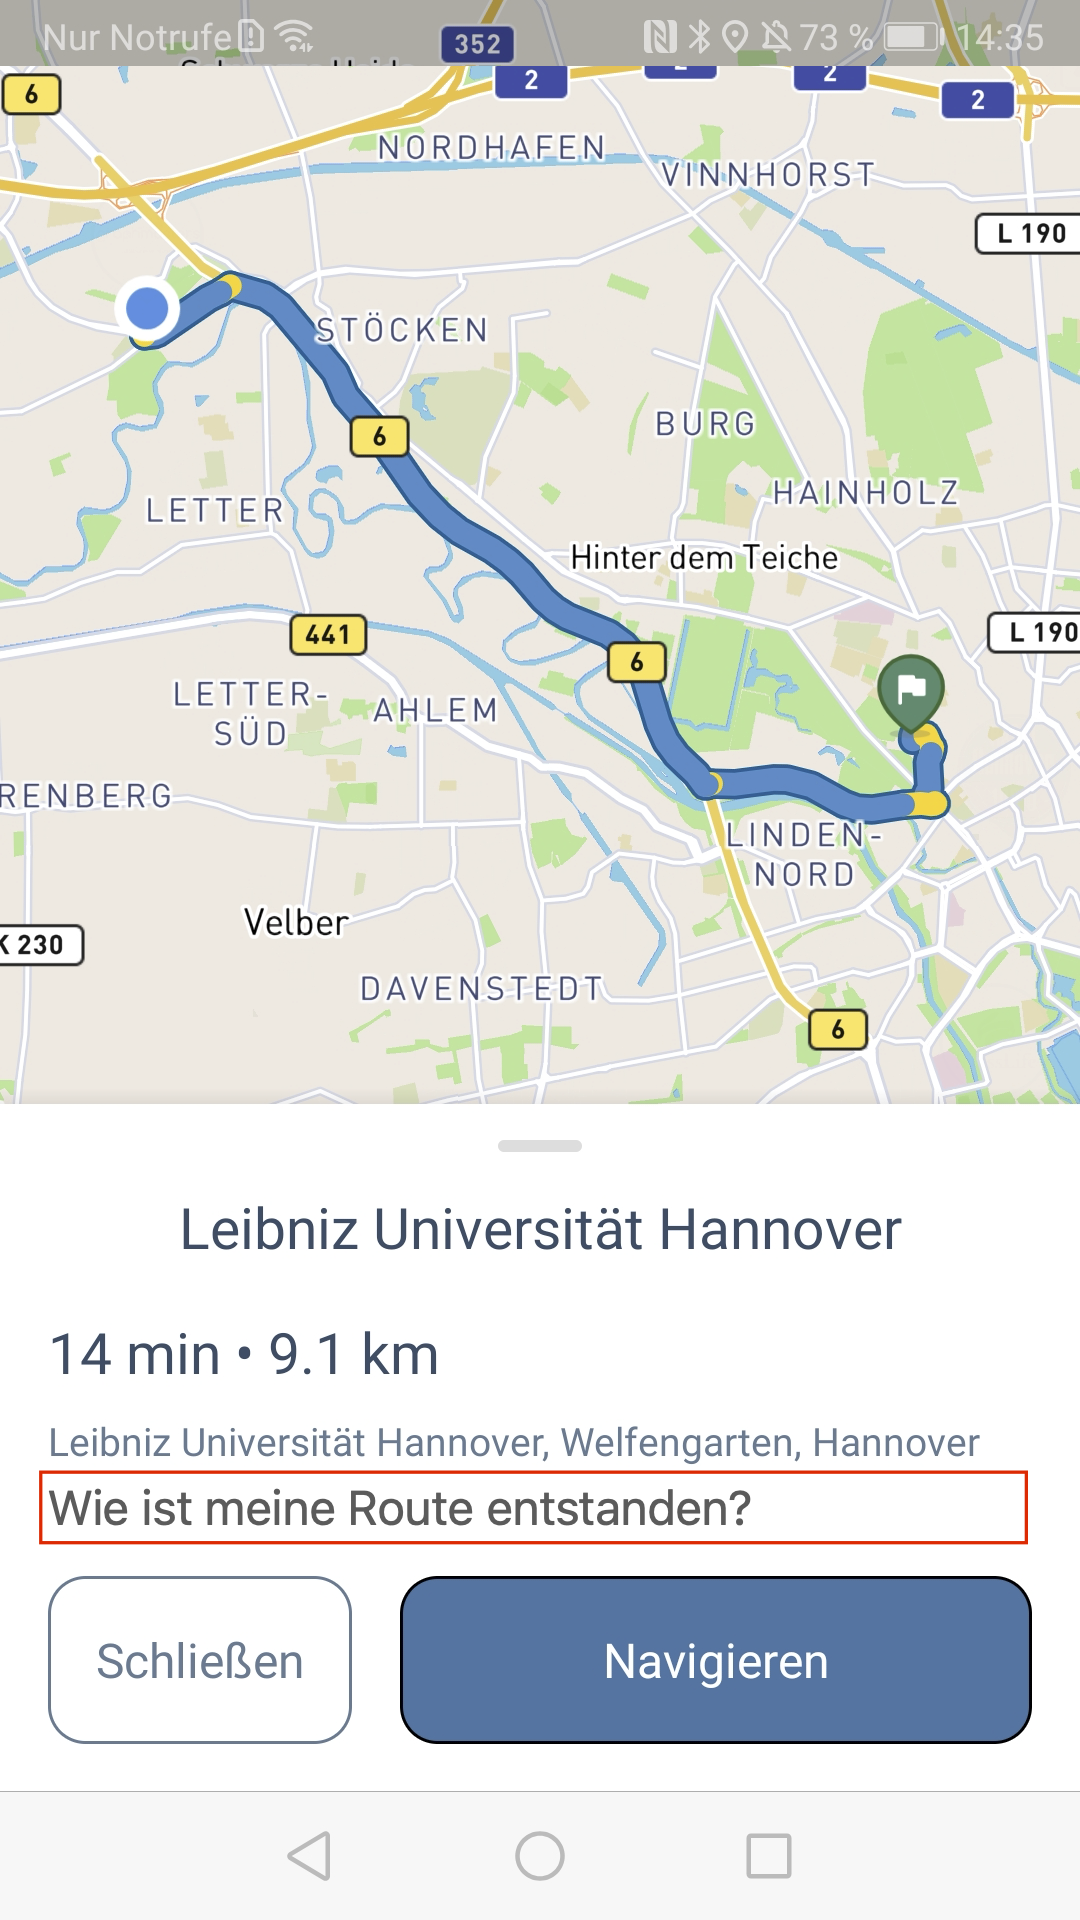
\includegraphics[width=.27\textwidth]{contents/06_model_evaluation/01_integration/res/02_routing_algorithm/prototype_1.png}
    }
    \hspace{.055\textwidth}
    \subfloat[Alternativer Prototyp zur Positionierung des Aufrufs der Erklärung]
    {
        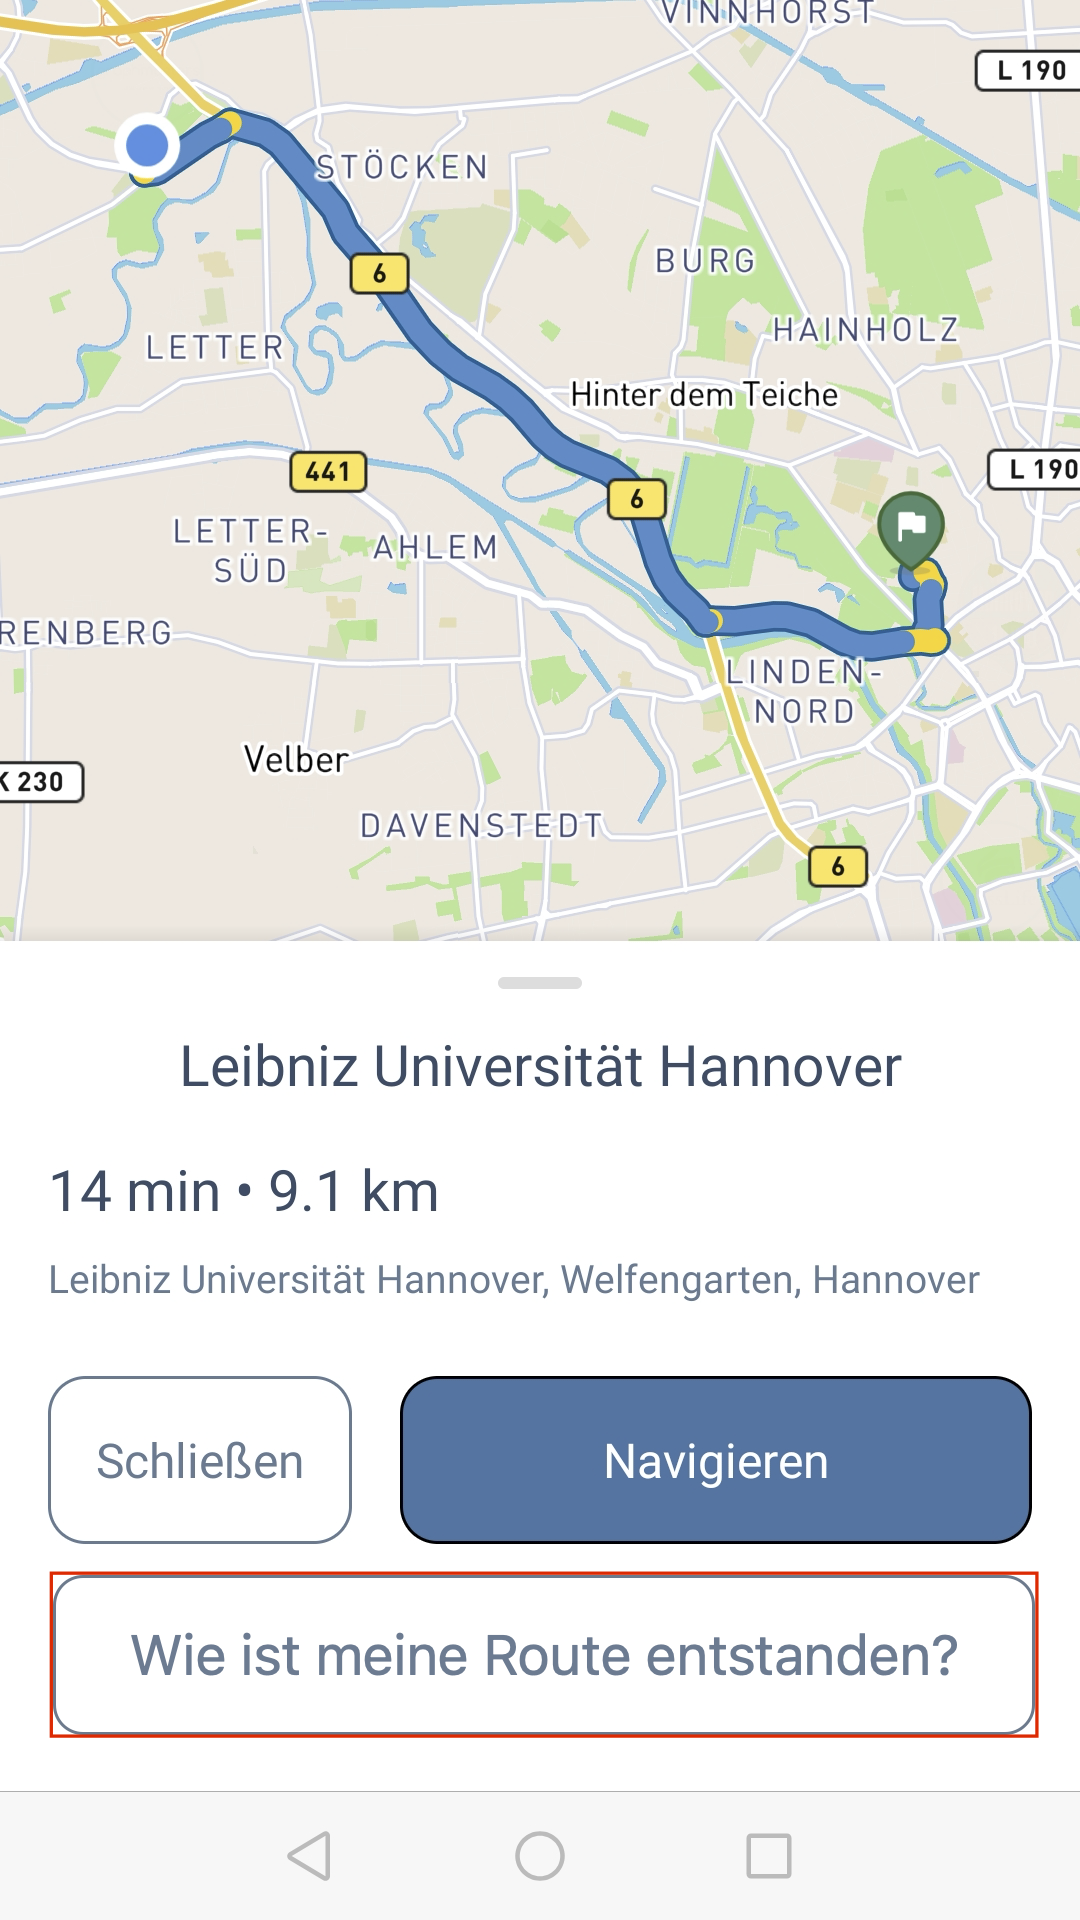
\includegraphics[width=.27\textwidth]{contents/06_model_evaluation/01_integration/res/02_routing_algorithm/prototype_2.png}
    }
    \hspace{.055\textwidth}
    \subfloat[Finales Design zur Positionierung des Aufrufs der Erklärung]
    {
        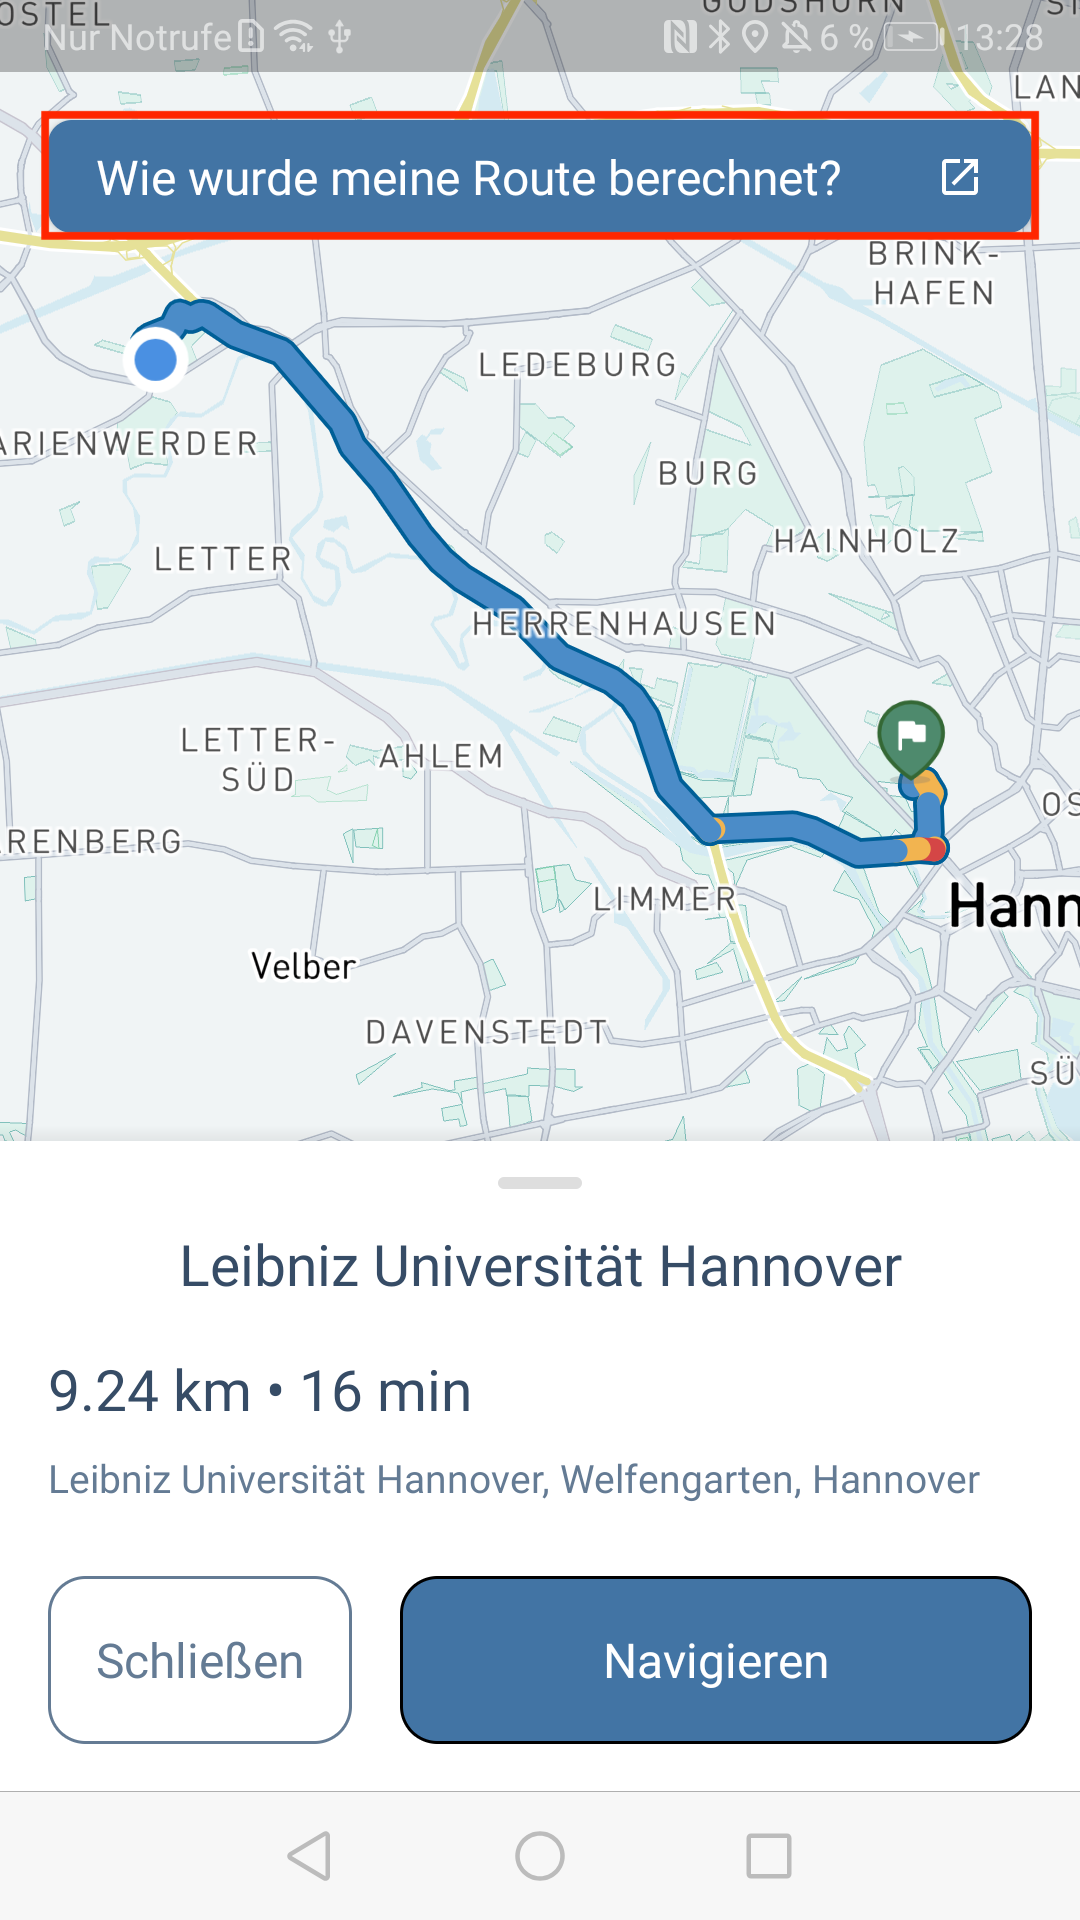
\includegraphics[width=.27\textwidth]{contents/06_model_evaluation/01_integration/res/02_routing_algorithm/final_1.png}
    }
    \caption{Prototyp und finale Designs für den Aufruf der Erklärung zu Einflüssen auf die Routenberechnung}
    \label{fig:prototype_routing_explanation}
\end{figure}

\subsubsection{Verkehrsaufkommen}
\label{sec:traffic_volume_definition}

\paragraph{[FR3]} \textit{NUNAV Navigation} muss den \textit{End Usern} während der Navigation Informationen zum Verkehrsgeschehen auf der aktuellen Route liefern.

Wie aus der Persona von Michael hervorgeht, wundert er sich zum Teil, warum \textit{NUNAV Navigation} aus seiner Sicht \glqq komische\grqq{} Routen vorschlägt. Ein Erklärungsansatz ist, das Verkehrsgeschehen auf der aktuellen Route anzuzeigen. Diese \textit{Context}-Information soll dabei helfen zu verstehen, warum \textit{NUNAV Navigation} andere Routen wählt. 

Dies ist allerdings nicht trivial, da die Berechnung des Verkehrsaufkommens und dessen subjektive Wahrnehmung der \textit{End User} nicht klar ist. Ein weiteres Problem ist, dass es nicht möglich ist, zu berechnen, welche Route für Nutzer auf der gleichen Strecke subjektiv als \glqq normal\grqq{} empfunden wird. Nachdem mehrere Lösungsansätze für dieses Problem in kleinen Runden bei \textit{Graphmasters} diskutiert wurden, wird als Lösung die Berechnung des Verhältnisses von durchschnittlicher Dauer der Route zu aktueller Dauer als Basiswert genommen. Die Daten werden dabei durch \textit{Nugraph} zur Verfügung gestellt und im Rahmen dieser Arbeit im \textit{BFF} auf die Stufen \glqq wenig Verkehr\grqq{}, \glqq mäßiger Verkehr\grqq{} und \glqq viel Verkehr\grqq{} abgebildet. Außerdem gibt es eine \glqq normale\grqq{} Verkehrssituation, in der den \textit{End Usern} keine Erklärung angezeigt wird. Die Abbildungsfunktion ist in den Zusatzmaterialien zu finden. Die Schwellwerte wurden intern durch Testfahrten ermittelt.

Die Informationen können \textit{End User} auf drei Wegen erhalten. Zunächst werden die Informationen in der Routenvorschau angezeigt. Dabei wird die Gesamtfahrzeit für die Route je nach Verkehrsaufkommen grün (wenig Verkehr), Standardtextfarbe (normaler Verkehr), orange (mäßiger Verkehr) und rot (viel Verkehr) dargestellt. Da im ersten Prototypen aufgefallen ist, dass die Farben alleine nicht aussagekräftig sind (siehe \autoref{fig:prototype_traffic_volume_route}, (a)), wurde zusätzlich ein kurzer Erklärungstext eingefügt (siehe \autoref{fig:prototype_traffic_volume_route}, (b)). Dieser ist bei \glqq normalem\grqq{} nicht zu sehen. So lernen die \textit{End User} mit der Zeit die Bedeutung der Farben. Eine Übersicht mit allen Prototypen ist in \autoref{sec:appendix_traffic_volume} zu finden.

Außerdem werden während der gesamten Navigation die Ankunftszeit und die Fahrzeit in der entsprechenden Farbe angezeigt und bei sich ändernder Verkehrssituation auch aktualisiert.

\begin{figure}[htb!]
    \centering
    \subfloat[Prototyp zur Darstellung des aktuellen Verkehrsaufkommens in der Routenvorschau]
    {
        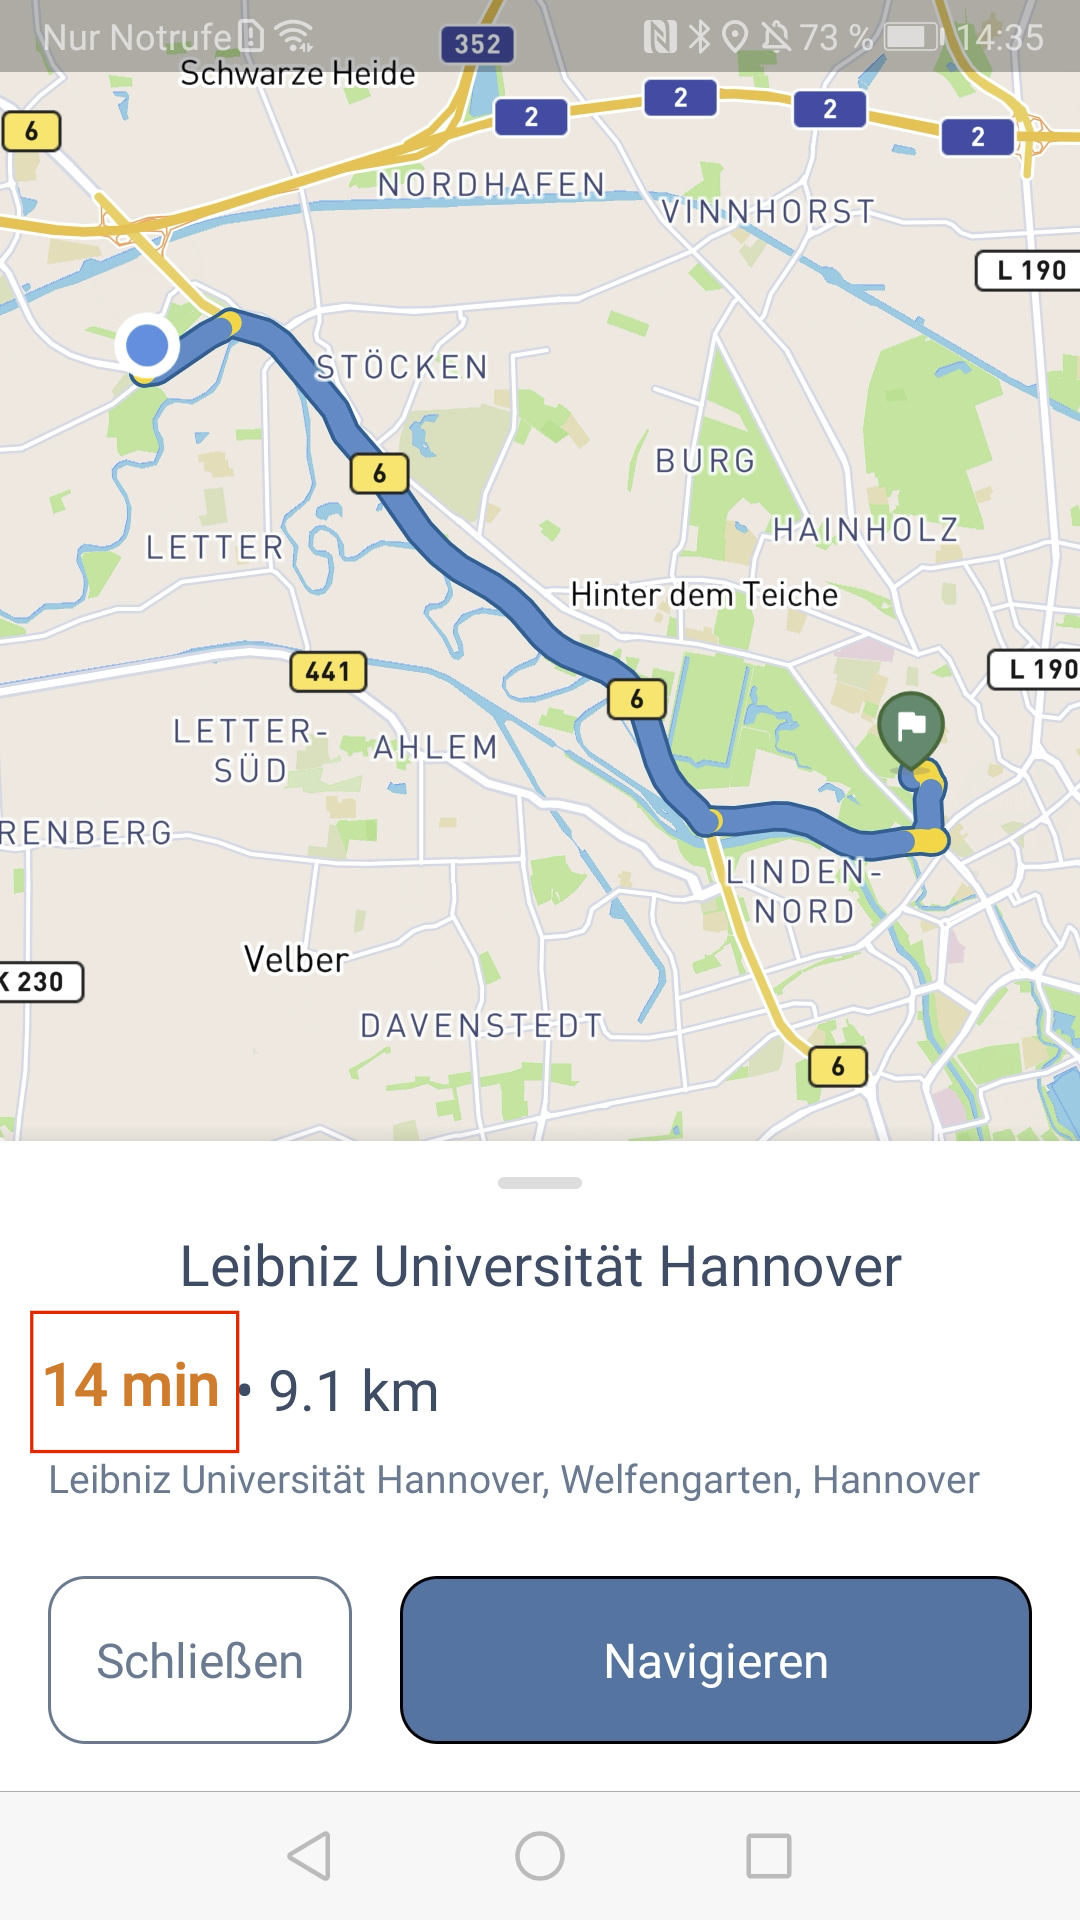
\includegraphics[width=.27\textwidth]{contents/06_model_evaluation/01_integration/res/03_traffic_volume/prototype_11.png}
    }
    \hspace{.055\textwidth}
    \subfloat[Finales Design zur Darstellung des aktuellen Verkehrsaufkommens in der Routenvorschau]
    {
        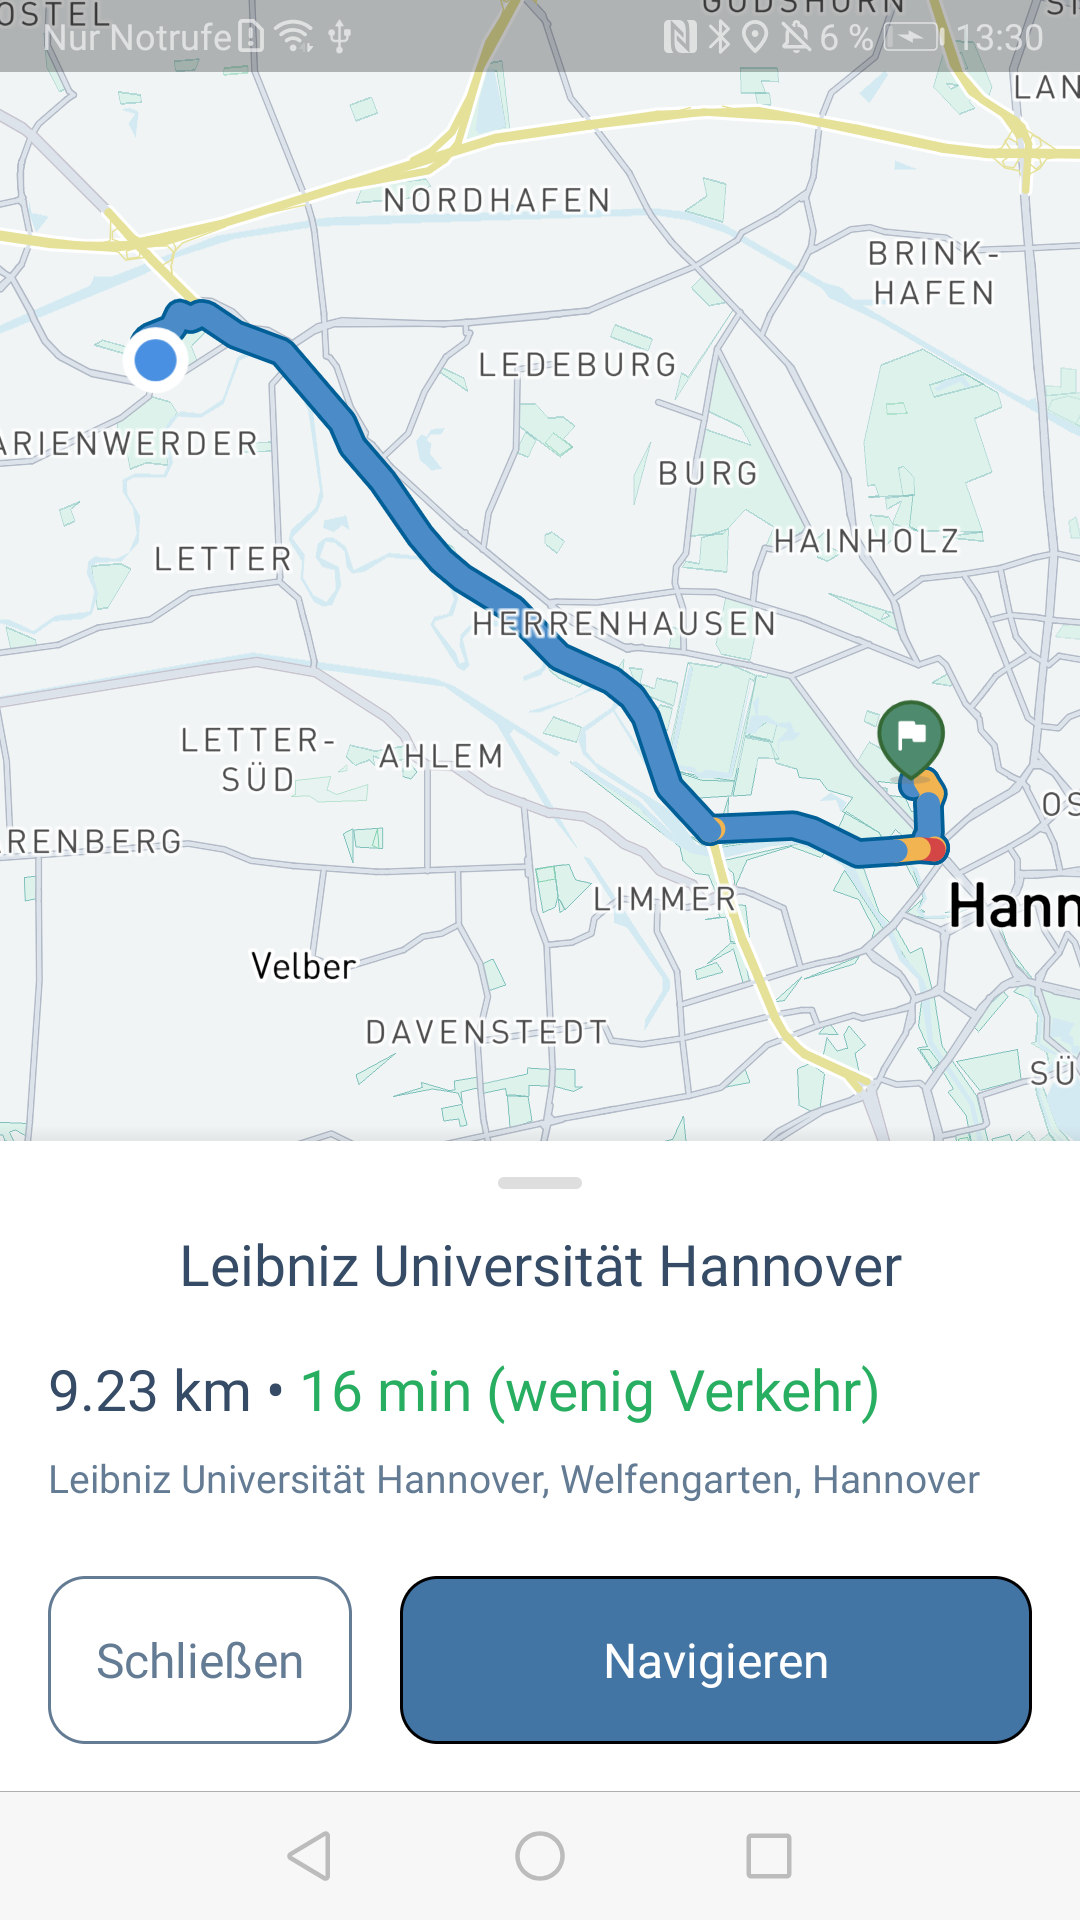
\includegraphics[width=.27\textwidth]{contents/06_model_evaluation/01_integration/res/03_traffic_volume/final_10.png}
    }
    \hspace{.055\textwidth}
    \subfloat[Finales Design zur Darstellung des aktuellen Verkehrsaufkommens während der Navigation]
    {
        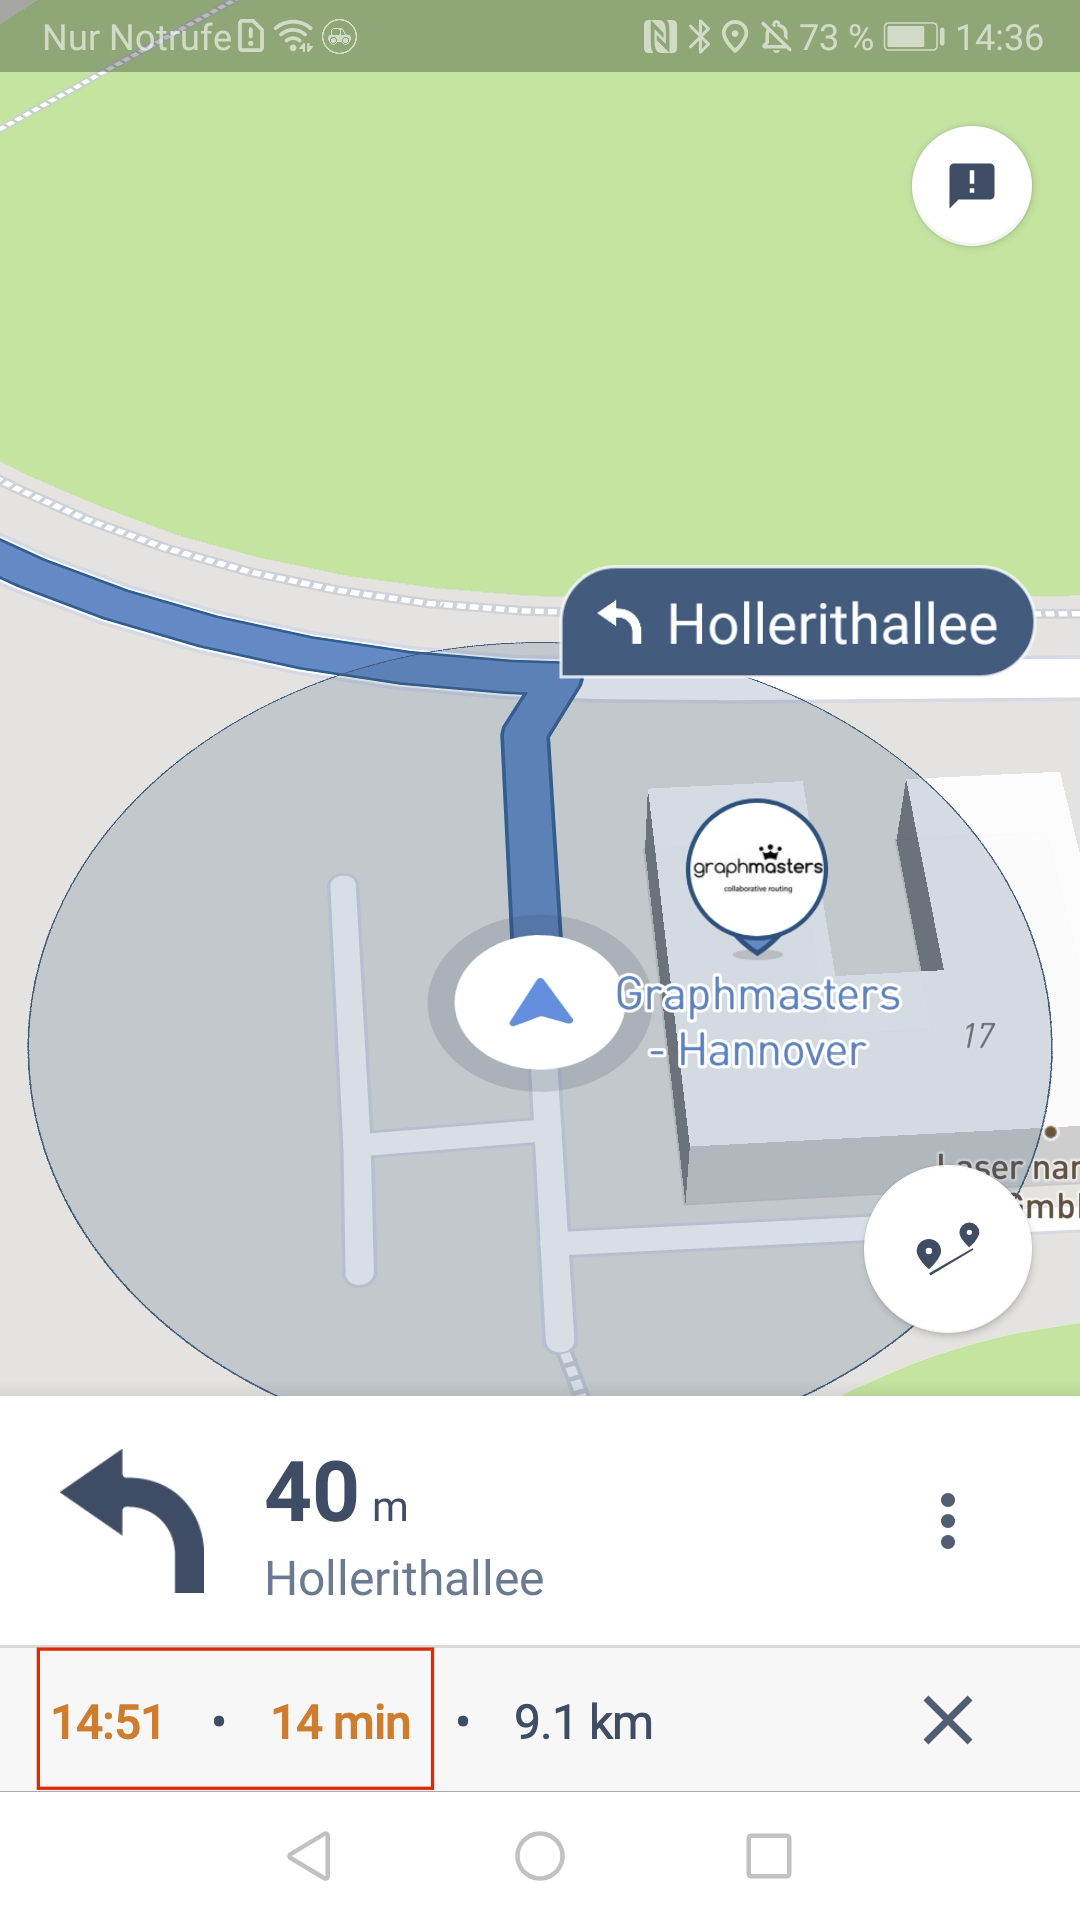
\includegraphics[width=.27\textwidth]{contents/06_model_evaluation/01_integration/res/03_traffic_volume/final_20.png}
    }
    \caption{Prototyp und finale Designs für die Erklärung zum kollaborativem Routing}
    \label{fig:prototype_traffic_volume_route}
\end{figure}

Des Weiteren ist das Sprachkommando, welches bei Start der Navigation gegeben wird, je nach Verkehrssituation unterschiedlich (siehe \autoref{tab:voice_commands_traffic_volume}).

\begin{table}[bht!]
    \begin{tabular}{p{.25\textwidth}p{.71\textwidth}}
        \hline
        Verkehrsaufkommen        & Sprachkommando \\
        \toprule
        wenig & Heute sind die Straßen frei. Du wirst dein Ziel <Zielname> um <Uhrzeit> erreichen. \\
        \tablerowspacing
        normal & Du wirst dein Ziel <Zielname> um <Uhrzeit> erreichen. \\
        \tablerowspacing
        mäßig & Da heute etwas mehr los ist, wirst du dein Ziel <Zielname> um <Uhrzeit> erreichen. \\
        \tablerowspacing
        viel & Da heute sehr viel los ist, wirst du dein Ziel <Zielname> um <Uhrzeit> erreichen. \\
        \toprule
    \end{tabular}
\caption{Sprachkommandos zum Start der Navigation abhängig von der Verkehrssituation}
\label{tab:voice_commands_traffic_volume}
\end{table}

\subsubsection{GPS-Qualität}
\label{sec:gps_accuracy_definition}

\paragraph{[FR4]} Wenn die Genauigkeit der Positionierung unzuverlässig ist, muss \textit{NUNAV Navigation} den \textit{End Usern} anzeigen, dass die Positionierung aktuell nicht zuverlässig ist.

Die letzte entwickelte Erklärung betrifft den Aspekt der \textit{Scrutability}. Ziel ist es \textit{End Usern} anzuzeigen, wenn sie sich aktuell auf die Position auf der Route nicht verlassen können. Dies ist zum Beispiel in Tunneln der Fall und besonders kritisch, wenn in Kürze ein Abbiege-Kommando erfolgt und somit an der falschen Stelle kommt. Bewusst wurde auf die technische Bezeichnung \glqq GPS\grqq{} verzichtet.

\begin{figure}[htb!]
    \centering
    \subfloat[Prototyp zum Design bei schlechtem GPS]
    {
        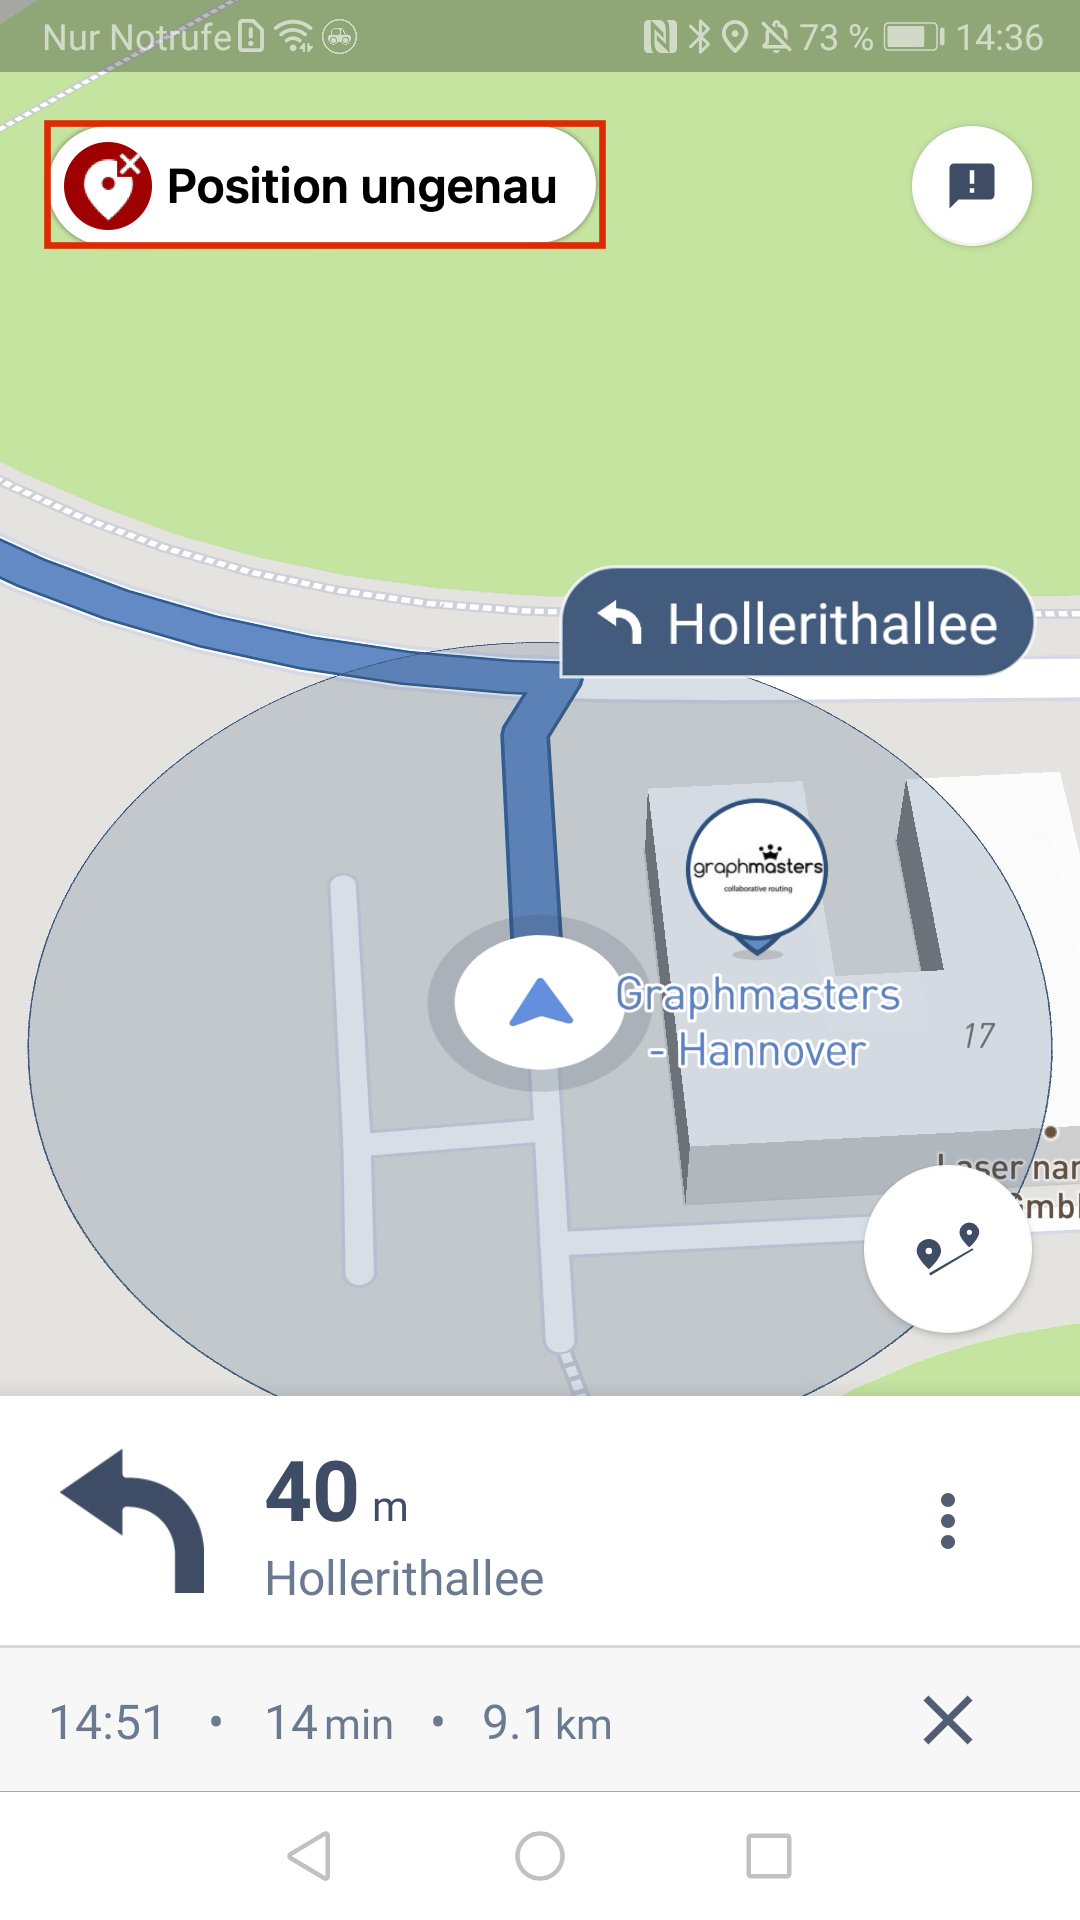
\includegraphics[width=.27\textwidth]{contents/06_model_evaluation/01_integration/res/04_position_accuracy/prototype_1.png}
    }
    \hspace{.055\textwidth}
    \subfloat[Finales Design bei schlechtem GPS]
    {
        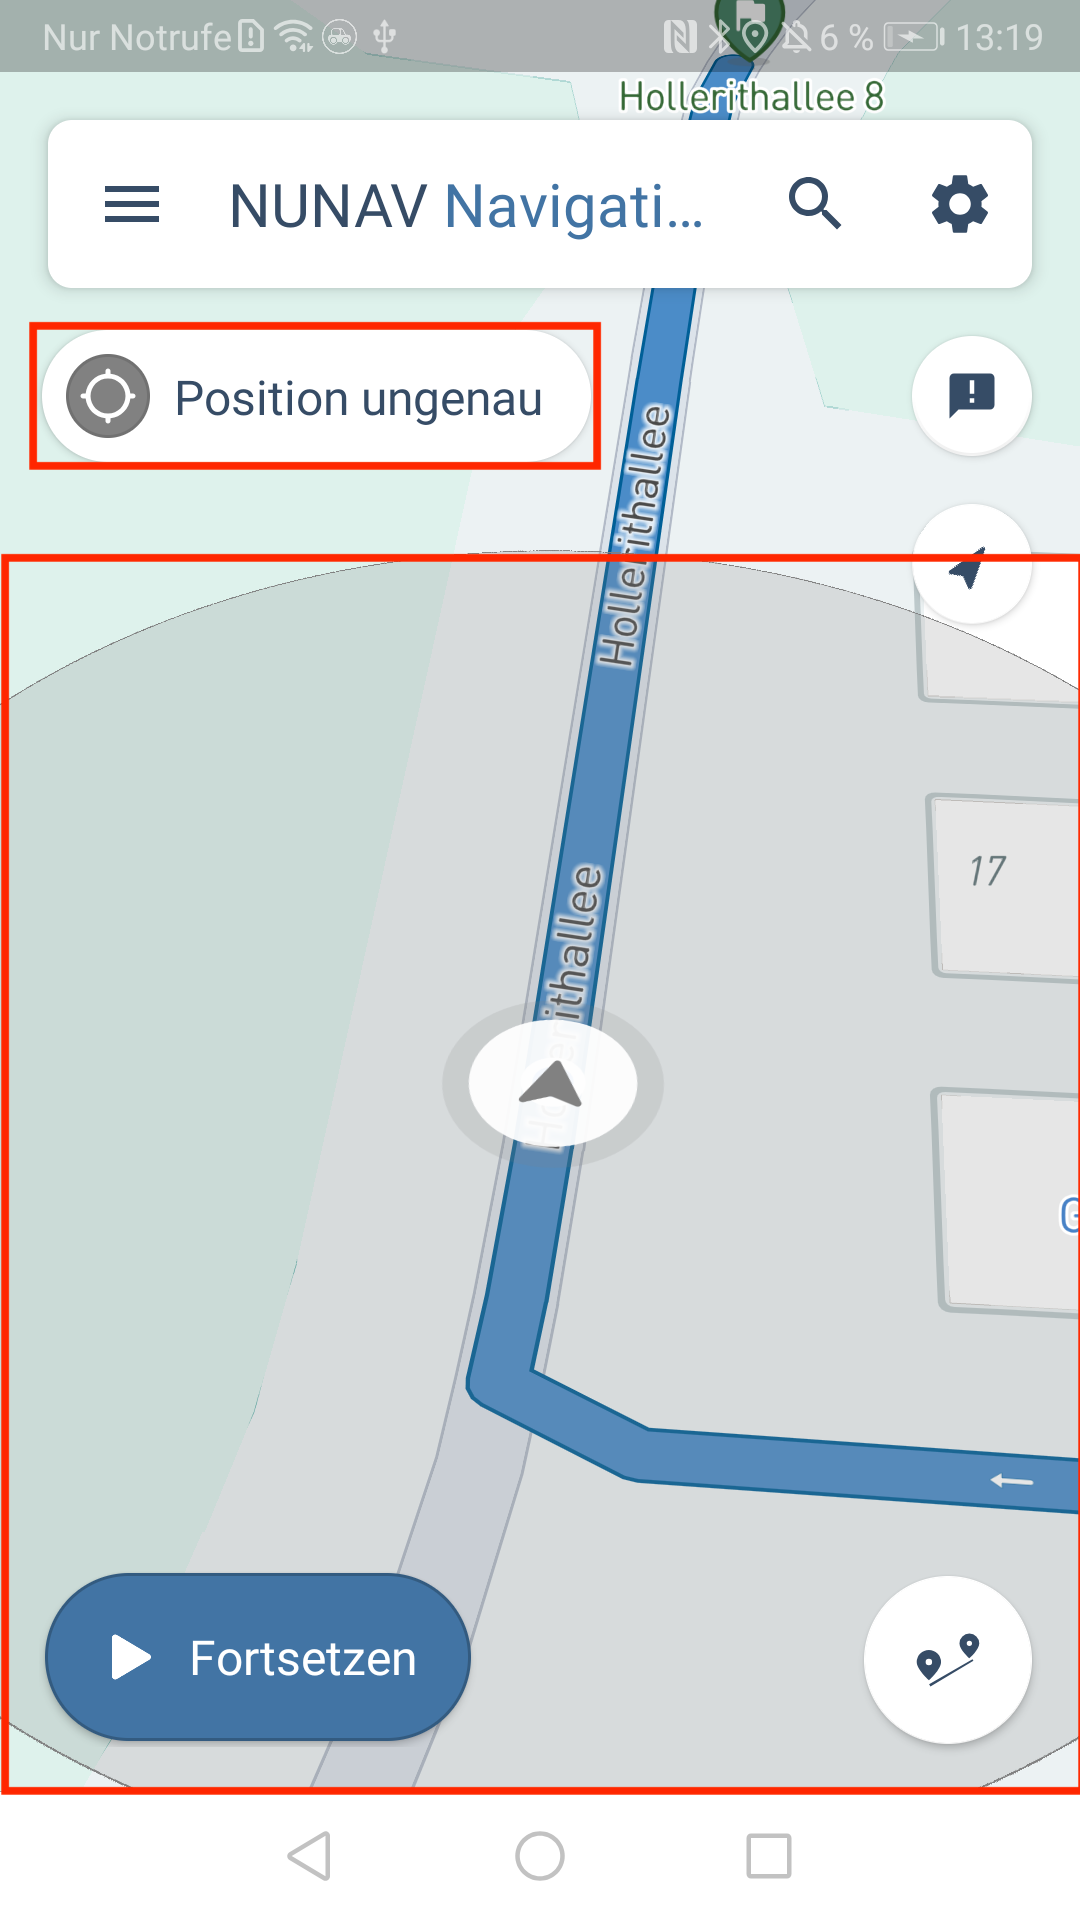
\includegraphics[width=.27\textwidth]{contents/06_model_evaluation/01_integration/res/04_position_accuracy/final_1.png}
    }
    \caption{Prototyp und finales Design für die Anzeige von schlechtem GPS während der Navigation}
    \label{fig:prototype_position_accuracy}
\end{figure}

Für die Entscheidung, wann das GPS ungenau ist, wurde innerhalb der \textit{NUNAV Navigation}-App ein neuer Algorithmus integriert, der diese trifft. Dabei spielt nicht nur die Genauigkeit, welche durch das GPS-Modul des Gerätes ermittelt wird, eine Rolle, sondern auch die Zeit, wann das letzte GPS-Update kam, da bei sehr schlechtem GPS keine Positionsupdates mehr vom Gerät geliefert werden. Der Algorithmus ist in den Zusatzmaterialien zu finden.

Als Design wurde im ersten Entwurf lediglich ein \textit{Growl} angezeigt und die Sprachansage \glqq Position ungenau\grqq{} ausgegeben. Insbesondere, wenn zum gleichen Zeitpunkt weitere \textit{Growls} angezeigt werden und die Sprachansagen vom \textit{End User} generell deaktiviert sind, hat sich die Sichtbarkeit bei Testfahrten als ungenügend herausgestellt. Daher wurde im finalen Entwurf zusätzlich das Positions-Icon auf der Karte und der Kreis, welcher die Genauigkeit der Position anzeigt, ausgegraut (siehe \autoref{fig:prototype_position_accuracy}, (b)).